\documentclass[landscape,paperwidth=40in,paperheight=34in]{baposter}

\usepackage{graphicx}
\usepackage{enumitem}
\usepackage{url}

% This prevents a \section being created for the bibliography
\renewcommand{\section}[2]{}%

\newcommand{\BI}{\begin{itemize}[itemsep=.05in,parsep=0in,leftmargin=.2in]}
\newcommand{\EI}{\end{itemize}}

\newcommand{\BE}{\begin{enumerate}[itemsep=.05in,parsep=0in,leftmargin=.2in]}
\newcommand{\EE}{\end{enumerate}}

\begin{document}

\begin{poster}{
  % key=value Options
  columns=4,
  headerheight=0.105\textheight,
  background=plain,
  bgColorOne=white,
  borderColor=black,
  headerColorOne=blue!20!white,
  headerColorTwo=blue!20!white,
  headershape=rounded,
  headerborder=none,
  headerfont=\Large\bf,
  textborder=none,
  boxshade=none
}{
  % Eye catcher

}{
  % Poster title
  CloudCoder --- A Web-Based Programming Exercise System
}{
  % Poster authors
  {\LARGE
  David Hovemeyer <{\tt dhovemey@ycp.edu}>, York College of Pennsylvania \\
  \vskip .05in
  Jaime Spacco <{\tt jspacco@knox.edu}>, Knox College}
}{
  % University logo(s)
  
\includegraphics[height=.75in]{images/YCPLogo}
  \hskip .1in
  
\includegraphics[height=.75in]{images/KnoxLogo}
}

  % Definition of boxes
  \headerbox{Programming is hard}{name=problem,column=0}{
    \vskip .1in
    {\raggedright\normalsize
    \BI
    \item {\bf Many students struggle} in intro programming courses
    \item Pass rates of 60\% (or worse!) are
      not unusual\cite{Bennedsen:2007:FRI:1272848.1272879}
    \item Students have difficulty learning syntax and basic concepts
    \item Exercises can help\cite{Kumar:2005:REE:1047124.1047422}
    \EI
    }
  }

  \headerbox{Exercises can help}{name=exercises,column=0,below=problem}{
    \vskip .1in
    {\raggedright\normalsize
    \BI
    \item Introduce syntax and concepts in {\bf small bites}
    \item {\bf Self-test exercises} to accompany reading assignments
    \item In-class {\bf assessment}
    \item Optional {\bf practice} for students who need it
    \EI
    }
  }

  \headerbox{Web-based systems}{name=systems,column=0,below=exercises}{
    \vskip .1in
    {\raggedright\normalsize
    \BI
    \item Students can {\bf access from anywhere} using a web browser,
      {\bf no software installation} (except on server)
    \item Lots of existing systems:
      \BI
      \item Free: CodingBat, PracticeIt!, CodeWrite, CodeAssessor, others
      \item Commercial: CodeLab, MyProgrammingLab, others
      \EI
    \item {\it Why create another?}
    \item Observation: a common model for pedagogical tools is
      \BE
      \item Implement it
      \item Publish paper(s) about it
      \item {\it Maybe} release software and get a few other
            institutions to use it
      \item Then it fades into disuse
      \EE
    \item Observation: adopting courseware has a significant cost
      \BI
      \item Need to convince instructors that a tool
            will be worth the effort
      \EI
    \EI
    }
  }

  \headerbox{Community!}{name=community,column=1}{
    \vskip .1in
    {\raggedright\normalsize
    Idea: {\bf crowdsourced exercises}
      \BI
      \item {\bf Users contribute exercises} under a permissive license
            (e.g., Creative Commons)
        \BI
        \item {\sc All your exercise are belong to us}
        \EI
      \item {\bf Central exercise repository} where exercises are published
      \item {\bf Open source software} that can be hosted anywhere
      \EI
    }
  }

  \headerbox{CloudCoder}{name=cloudcoder,column=1,below=community}{
    \vskip .1in
    {\raggedright\normalsize
    \BI
      \item Website: \url{http://cloudcoder.org}
      \item {\bf Open source} (AGPL v3)
      \item Supports {\bf C}, {\bf Java}, and {\bf Python} exercises
      \item (Relatively) {\bf easy to host}
        \BI
        \item It's a Java web application
        \item Single-jar deployment using Jetty
        \EI
      \item Requires two {\bf Linux servers}:
        \BI
        \item One for {\bf webapp}, needs a MySQL database
        \item One (or more) to {\bf build/test} student submissions
        \EI
      \item {\bf Exercise repository}:
            \url{https://cloudcoder.org/repo}
        \BI
        \item {\bf Simple import/export} of exercises
        \item {\bf Browsing/searching} to find exercises
        \EI
    \EI
    }
  }

  \headerbox{Experiences}{name=experiences,column=1,below=cloudcoder}{
    \vskip .1in
    {\raggedright\normalsize
    \BI
    \item Used at 4 institutions (York College, Knox College, Canisius College,
          University of Auckland)
    \item Exercise repository: small but growing
    \item From a student: ``Every time I see that green bar makes me WAAAYYY too happy''
    \EI
    }
  }

  \headerbox{Screenshot}{name=screenshot,column=2,span=2}{
    \vskip .1in
    \begin{center}
    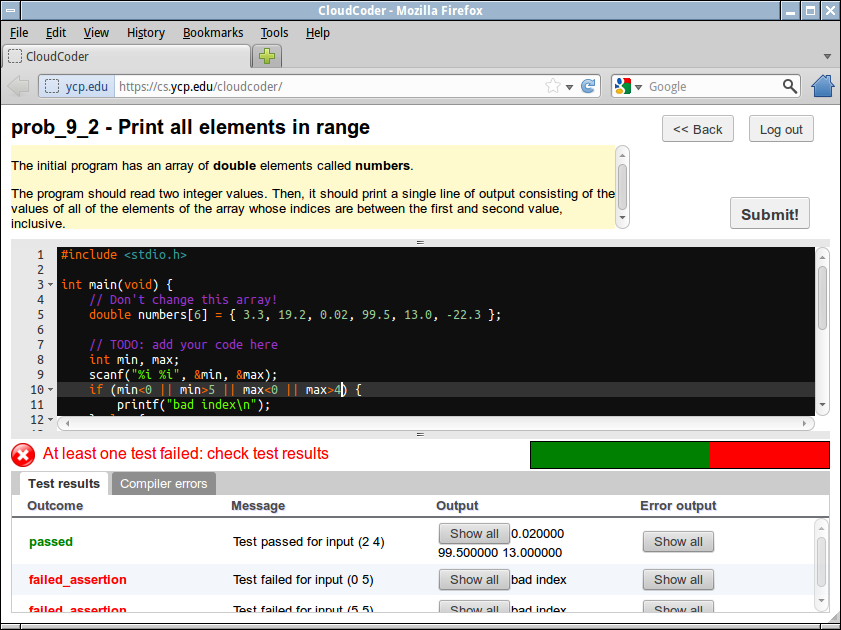
\includegraphics[width=5.25in]{images/ccScreenshot}
    \end{center}
  }

  \headerbox{We need your help!}{name=needhelp,column=2,below=screenshot}{
    \vskip .1in
    {\raggedright\normalsize
    \BI
    \item {\bf Try it out}!
    \item {\bf Use our exercises}!
    \item {\bf Share your exercises}!
    \EI
    }
  }

  \headerbox{Results?}{name=results,column=2,below=needhelp}{
    \vskip .1in
    {\raggedright\normalsize
    Can CloudCoder improve learning?\\
    {\bf We don't know}!
      \BI
      \item Spring 2013: {\bf full study} using CloudCoder exercises
            for self-test, in-class assessment, and remediation/practice
      \item At York College and other institutions
      \item {\bf Join us}!  We are actively seeking collaborators
      \EI
    }
  }

  \headerbox{References}{name=references,column=3,below=screenshot}{
    \vskip .1in
    {\small
    \bibliographystyle{plain}
    \bibliography{poster}
    }
  }

  \headerbox{Support}{name=support,column=3,below=references}{
    \vskip .1in
    {\small
    Supported by a SIGCSE special projects grant, May 2012
    }
  }

\end{poster}

\end{document}
